\documentclass[aspectratio=43,t]{beamer}
% \documentclass[aspectratio=169]{beamer}

% Title --------------------------------------------
\title{Generalized Imputation Estimators for Factor Models}
\date{\today}
\author{
Nicholas Brown and Kyle Butts
}

% xcolor and define colors -------------------------
\usepackage{xcolor}

% https://www.viget.com/articles/color-contrast/
\definecolor{purple}{HTML}{695693}
\definecolor{navy}{HTML}{567293}
\definecolor{ruby}{HTML}{9a2515}
\definecolor{alice}{HTML}{107895}
\definecolor{daisy}{HTML}{EBC944}
\definecolor{coral}{HTML}{F26D21}
\definecolor{kelly}{HTML}{829356}
\definecolor{cranberry}{HTML}{E64173}
\definecolor{jet}{HTML}{131516}
\definecolor{asher}{HTML}{555F61}
\definecolor{slate}{HTML}{314F4F}

% Main theme colors
\definecolor{accent}{HTML}{107895}
\definecolor{accent2}{HTML}{E64173}

\newcommand\navy[1]{{\color{navy}#1}}
\newcommand\purple[1]{{\color{purple}#1}}
\newcommand\kelly[1]{{\color{kelly}#1}}
\newcommand\ruby[1]{{\color{ruby}#1}}
\newcommand\alice[1]{{\color{alice}#1}}
\newcommand\daisy[1]{{\color{daisy}#1}}
\newcommand\coral[1]{{\color{coral}#1}}
\newcommand\cranberry[1]{{\color{cranberry}#1}}
\newcommand\slate[1]{{\color{slate}#1}}
\newcommand\jet[1]{{\color{jet}#1}}
\newcommand\asher[1]{{\color{asher}#1}}

\newcommand\bgNavy[1]{{\colorbox{navy!80!white}{#1}}}
\newcommand\bgPurple[1]{{\colorbox{purple!80!white}{#1}}}
\newcommand\bgKelly[1]{{\colorbox{kelly!80!white}{#1}}}
\newcommand\bgRuby[1]{{\colorbox{ruby!80!white}{#1}}}
\newcommand\bgAlice[1]{{\colorbox{alice!80!white}{#1}}}
\newcommand\bgDaisy[1]{{\colorbox{daisy!80!white}{#1}}}
\newcommand\bgCoral[1]{{\colorbox{coral!80!white}{#1}}}
\newcommand\bgCranberry[1]{{\colorbox{cranberry!80!white}{#1}}}


% Beamer Options -------------------------------------

% Background
\setbeamercolor{background canvas}{bg = white}

% Change text margins
\setbeamersize{text margin left = 15pt, text margin right = 15pt} 

% \alert
\setbeamercolor{alerted text}{fg = accent2}

% Frame title
\setbeamercolor{frametitle}{bg = white, fg = jet}
\setbeamercolor{framesubtitle}{bg = white, fg = accent}
\setbeamerfont{framesubtitle}{size = \small, shape = \itshape}

% Block
\setbeamercolor{block title}{fg = white, bg = accent2}
\setbeamercolor{block body}{fg = jet, bg = jet!10!white}

% Title page
\setbeamercolor{title}{fg = jet}
\setbeamercolor{subtitle}{fg = accent}

%% Custom \maketitle and \titlepage
\setbeamertemplate{title page}
{
    %\begin{centering}
        \vspace{20mm}
        {\Large \usebeamerfont{title}\usebeamercolor[fg]{title}\inserttitle}\\ \vskip0.25em%
        \ifx\insertsubtitle\@empty%
        \else%
          {\usebeamerfont{subtitle}\usebeamercolor[fg]{subtitle}\insertsubtitle\par}%
        \fi% 
        {\vspace{10mm}\insertauthor}\\
        {\color{asher}\small{\insertdate}}\\
    %\end{centering}
}

% Table of Contents
\setbeamercolor{section in toc}{fg = accent!70!jet}
\setbeamercolor{subsection in toc}{fg = jet}

% Button 
\setbeamercolor{button}{bg = accent}

% Remove navigation symbols
\setbeamertemplate{navigation symbols}{}

% Table and Figure captions
\setbeamercolor{caption}{fg=jet!70!white}
\setbeamercolor{caption name}{fg=jet}
\setbeamerfont{caption name}{shape = \itshape}

% Bullet points

%% Fix left-margins
\settowidth{\leftmargini}{\usebeamertemplate{itemize item}}
\addtolength{\leftmargini}{\labelsep}

%% enumerate item color
\setbeamercolor{enumerate item}{fg = accent}
\setbeamerfont{enumerate item}{size = \small}
\setbeamertemplate{enumerate item}{\insertenumlabel.}

%% itemize
\setbeamercolor{itemize item}{fg = accent!70!white}
\setbeamerfont{itemize item}{size = \small}
\setbeamertemplate{itemize item}[circle]

%% right arrow for subitems
\setbeamercolor{itemize subitem}{fg = accent!60!white}
\setbeamerfont{itemize subitem}{size = \small}
\setbeamertemplate{itemize subitem}{$\rightarrow$}

\setbeamertemplate{itemize subsubitem}[square]
\setbeamercolor{itemize subsubitem}{fg = jet}
\setbeamerfont{itemize subsubitem}{size = \small}

% References

%% Bibliography Font, roughly matching aea
\setbeamerfont{bibliography item}{size = \footnotesize}
\setbeamerfont{bibliography entry author}{size = \footnotesize, series = \bfseries}
\setbeamerfont{bibliography entry title}{size = \footnotesize}
\setbeamerfont{bibliography entry location}{size = \footnotesize, shape = \itshape}
\setbeamerfont{bibliography entry note}{size = \footnotesize}

\setbeamercolor{bibliography item}{fg = jet}
\setbeamercolor{bibliography entry author}{fg = accent!60!jet}
\setbeamercolor{bibliography entry title}{fg = jet}
\setbeamercolor{bibliography entry location}{fg = jet}
\setbeamercolor{bibliography entry note}{fg = jet}

%% Remove bibliography symbol in slides
\setbeamertemplate{bibliography item}{}





% Links ----------------------------------------------

\usepackage{hyperref}
\hypersetup{
  colorlinks = true,
  linkcolor = accent2,
  filecolor = accent2,
  urlcolor = accent2,
  citecolor = accent2,
}


% Line spacing --------------------------------------
\usepackage{setspace}
\setstretch{1.3}


% \begin{columns} -----------------------------------
\usepackage{multicol}


% Fonts ---------------------------------------------
% Beamer Option to use custom fonts
\usefonttheme{professionalfonts}

% \usepackage[utopia, smallerops, varg]{newtxmath}
% \usepackage{utopia}
\usepackage[sfdefault,light]{roboto}

% Small adjustments to text kerning
\usepackage{microtype}



% Remove annoying over-full box warnings -----------
\vfuzz2pt 
\hfuzz2pt


% Table of Contents with Sections
\setbeamerfont{myTOC}{series=\bfseries, size=\Large}
\AtBeginSection[]{
        \frame{
            \frametitle{Roadmap}
            \tableofcontents[current]   
        }
    }


% References ----------------------------------------
\usepackage[
    citestyle= authoryear,
    style = authoryear,
    natbib = true, 
    backend = biber
]{biblatex}

% Smaller font-size for references
\renewcommand*{\bibfont}{\small}

% Remove "In:"
\renewbibmacro{in:}{}

% Color citations for slides
\newenvironment{citecolor}
    {\footnotesize\begin{color}{accent2}}
    {\end{color}}

\newcommand{\citetcolor}[1]{{\footnotesize\textcolor{gray}{\citet{#1}}}}
\newcommand{\citepcolor}[1]{{\footnotesize\textcolor{gray}{\citep{#1}}}}

% Tables -------------------------------------------
% Tables too big
% \begin{adjustbox}{width = 1.2\textwidth, center}
\usepackage{adjustbox}
\usepackage{array}
\usepackage{threeparttable, booktabs, adjustbox}
    
% Fix \input with tables
% \input fails when \\ is at end of external .tex file

\makeatletter
\let\input\@@input
\makeatother

% Tables too narrow
% \begin{tabularx}{\linewidth}{cols}
% col-types: X - center, L - left, R -right
% Relative scale: >{\hsize=.8\hsize}X/L/R
\usepackage{tabularx}
\newcolumntype{L}{>{\raggedright\arraybackslash}X}
\newcolumntype{R}{>{\raggedleft\arraybackslash}X}
\newcolumntype{C}{>{\centering\arraybackslash}X}

% Figures

% \imageframe{img_name} -----------------------------
% from https://github.com/mattjetwell/cousteau
\newcommand{\imageframe}[1]{%
    \begin{frame}[plain]
        \begin{tikzpicture}[remember picture, overlay]
            \node[at = (current page.center), xshift = 0cm] (cover) {%
                \includegraphics[keepaspectratio, width=\paperwidth, height=\paperheight]{#1}
            };
        \end{tikzpicture}
    \end{frame}%
}

% subfigures
\usepackage{subfigure}




% Highlight slide -----------------------------------
% \begin{transitionframe} Text \end{transitionframe}
% from paulgp's beamer tips
\newenvironment{transitionframe}{
    \setbeamercolor{background canvas}{bg=accent!60!black}
    \begin{frame}\color{accent!10!white}\LARGE\centering
}{
    \end{frame}
}


% Table Highlighting --------------------------------
% Create top-left and bottom-right markets in tabular cells with a unique matching id and these commands will outline those cells

\usepackage[beamer,customcolors]{hf-tikz}
\usetikzlibrary{calc}
\usetikzlibrary{fit,shapes.misc}

\usepackage{pgfplots}
\pgfplotsset{compat=newest}
\usepgfplotslibrary{groupplots}
\usepgfplotslibrary{polar}
\usepgfplotslibrary{smithchart}
\usepgfplotslibrary{statistics}
\usepgfplotslibrary{dateplot}
\usepgfplotslibrary{ternary}
\usetikzlibrary{arrows.meta}
\usetikzlibrary{backgrounds}
\usepgfplotslibrary{patchplots}
\usepgfplotslibrary{fillbetween}
\pgfplotsset{%
    layers/standard/.define layer set={%
        background,axis background,axis grid,axis ticks,axis lines,axis tick labels,pre main,main,axis descriptions,axis foreground%
    }{
        grid style={/pgfplots/on layer=axis grid},%
        tick style={/pgfplots/on layer=axis ticks},%
        axis line style={/pgfplots/on layer=axis lines},%
        label style={/pgfplots/on layer=axis descriptions},%
        legend style={/pgfplots/on layer=axis descriptions},%
        title style={/pgfplots/on layer=axis descriptions},%
        colorbar style={/pgfplots/on layer=axis descriptions},%
        ticklabel style={/pgfplots/on layer=axis tick labels},%
        axis background@ style={/pgfplots/on layer=axis background},%
        3d box foreground style={/pgfplots/on layer=axis foreground},%
    },
}

% To set the hypothesis highlighting boxes red.
\newcommand\marktopleft[1]{%
    \tikz[overlay,remember picture] 
        \node (marker-#1-a) at (0,1.5ex) {};%
}
\newcommand\markbottomright[1]{%
    \tikz[overlay,remember picture] 
        \node (marker-#1-b) at (0,0) {};%
    \tikz[accent!80!jet, ultra thick, overlay, remember picture, inner sep=4pt]
        \node[draw, rectangle, fit=(marker-#1-a.center) (marker-#1-b.center)] {};%
}


% Custom Math Definitions ------------------------------------------------------

\global\long\def\expec#1{\mathbb{E}\left[#1\right]}%
\newcommand{\condexpec}[2]{\mathbb{E}\left[#1 \ \vert \ #2\right]}
\global\long\def\prob#1{\mathbb{P}\left[#1\right]}%
\global\long\def\var#1{\mathrm{Var}\left[#1\right]}%
\global\long\def\cov#1{\mathrm{Cov}\left[#1\right]}%
\global\long\def\one{\mathbf{1}}%

% \graphicspath{../../figures/}

% Set-up Bibliography ------------------------------
\addbibresource{references.bib}
\usepackage{bm}
\usepackage{adjustbox}

\begin{document}

% ------------------------------------------------------------------------------
\begin{frame}
\maketitle

% \vspace{2.5mm}
% {}
\end{frame}
% ------------------------------------------------------------------------------

\begin{frame}{Introduction}
    We are interested in effects of a treatment/intervention. 

    \vspace{.5cm}

    \textbf{Notation:}

    Observed outcomes have two potential states:
    \begin{itemize}
        \item Treated potential outcomes $y_{it}(1)$.
        \item Untreated potential outcomes $y_{it}(0)$.
    \end{itemize}


    \bigskip   
    The \textbf{treatment effect}, at time $t$ is 
    \begin{equation}
        \tau_{it} = y_{it}(1) - \coral{y_{it}(0)}
    \end{equation}

    
\end{frame}

\begin{frame}{Introduction}
      We aim to estimate average treatment effects on the treated, e.g. overall effect and event-study effects
      \begin{itemize}
        \item A particular form of \textbf{impulse response} with a binary treatment \citep{jorda2005estimation}
      \end{itemize}

      Our goal is to `impute' $\coral{y_{it}(0)}$; that is, estimate what the treated units outcomes would have been without treatment.
\end{frame}

\begin{frame}{TWFE and Parallel Trends}
    $$
    \coral{y_{it}(0)} = \mu_i + \theta_t + u_{it}
    $$
    
    \bigskip
    Under this model, we need a parallel trends assumption that the time shocks are experienced commonly between the control units and the treated units ($\theta_t$ is constant)
    
    \bigskip\pause
    This is often undesirable, units select into treatment based on their economic trends all the time!
\end{frame}

\begin{frame}{Example:}
    Walmart choses where to open new stores in the 90s.
    \begin{itemize}
        \item Interested on the labor market impacts
    \end{itemize}

    \vspace{.5cm} \pause

    \textbf{Untreated Model 1:} $\text{employment}_{it}(0) = \text{macro}_t + \text{county}_i + u_{it}$.
    \begin{itemize}
        \item We would need to assume that treated counties and control counties are on the same trend
    \end{itemize}

    \vspace{.5 cm}\pause 

    \textbf{Untreated Model 2:} $\text{employment}_{it}(0) = \text{macro}_t * \text{county}_i + u_{it}$.
    \begin{itemize}
        \item Under this model, we can allow treated counties to have differential exposure to the macro shocks (e.g. manufacturing share)
    \end{itemize}
\end{frame}


\begin{frame}{Empirical Macro}
  \textbf{Large policy changes}: 
  \begin{itemize}
    \item \citet{ramey2016macroeconomic} gives examples of technological shocks, monetary policy shocks, and fiscal shocks
    \item e.g. \citet{leblebiciouglu2020credit} look at banking deregulation on the labor share using an event-study regression
  \end{itemize}

  \smallskip
  \textbf{Abnormal returns}: 
  \begin{itemize}
    \item \citet{kothari2007econometrics} review estimation difficulties
    \item Our method works in short-panels; helps with problems of structural breaks in long time-series
    \item Synthetic control fails even in reasonably long panels if there are highly autocorrelated errors
  \end{itemize}
\end{frame}

\begin{frame}{Empirical Macro}
  \textbf{Marginal propensity to consume}:
  \begin{itemize}
    \item \citet{broda2014economic} and \citet{parker2013consumer} estimate event-study analysis of 2008 stimulus payments.
    
    \item Estimation is complicated if payments are targeted based on economic status
  \end{itemize}

  \smallskip
  \textbf{Fiscal multipliers}:
  \begin{itemize}
    \item Estimated via impulse response: \citet{ilzetzki2013big} and \citet{brinca2016fiscal}
    \item Again, targeting of fiscal stimulus is non-random
  \end{itemize}
\end{frame}

\section{Generalized Imputation Estimators}

\begin{frame}{Model}
    $N$ individuals observed for $T$ times periods.
    \begin{itemize}
        \item Treatment begins \textbf{after} period $T_0$ (ignoring staggered treatment timing for this presentation).
        \item $N_1$ treated individuals, $N_0$ untreated individuals.
    \end{itemize}
    
    \pause
    \bigskip
    Untreated potential outcomes are given by a \textbf{factor model}:
    \begin{equation}
        y_{it}(0) = \mu_i + \theta_t + \bm f_t' \bm \gamma_i + u_{it}
    \end{equation}
    
    \vspace{-3mm}
    \begin{itemize}
        \item $\bm f_t$: $p \times 1$ vector of common factors.
        \item $\bm \gamma_i$: $p \times 1$ vector of individual factor loadings.
        \item Nests the common TWFE model ($\bm \gamma_i = 0$). 
    \end{itemize}
\end{frame}

\begin{frame}{Assumptions}
    \textbf{Arbitrary Treatment Effects:}
    \begin{equation}
        y_{it}(1) = y_{it}(0) + \tau_{it}
    \end{equation}


    \bigskip\pause
    \textbf{No Anticipation:}
    $$
      y_{it}(0) = y_{it} \ \text{if}\  d_{it} = 0
    $$

    \begin{itemize}
        \item Treated units do not change their behavior before treatment.
        \item Can estimate and test for limited anticipation effects in our framework. 
    \end{itemize}
\end{frame}

\begin{frame}{Assumptions}
    \textbf{Selection into Treatment:}
    \begin{equation*}
        \condexpec{u_{it}}{\mu_i, \bm \gamma_i, D_i} = 0
    \end{equation*}
    
    \begin{itemize}
        \item \textbf{Mean Model:} $\condexpec{y_{it}(0)}{\mu_i, \bm \gamma_i, D_i} = \mu_i + \theta_t + \bm f_t' \condexpec{\bm \gamma_i}{D_i}$.

        \item Allows selection into treatment based on level and interactive fixed effects, but not idiosyncratic shocks
    \end{itemize}
\end{frame}

\begin{frame}{Selection into Treatment and Parallel Trends}
    In the two period case ($t = 1, 0$) consider the difference-in-differences estimand:
    \begin{align*}
        &\condexpec{y_{i1}(1) - y_{i0}(0)}{D_i = 1} - \condexpec{y_{i1}(0) - y_{i0}(0)}{D_i = 0} \\ \pause
        &= \condexpec{\tau_{it}}{D_i = 1} + \bm f_t' \big( \condexpec{\bm \gamma_i}{D_i = 1} - \condexpec{\bm \gamma_i}{D_i = 0} \big) 
    \end{align*}
    
    \bigskip \pause
    This last term makes parallel trends not hold! That is, differential exposure to macroeconomic shocks violates parallel trends!
\end{frame}

\begin{frame}{Identification under a factor model}
    There are many estimators for treatment effects under factor models:
    \begin{enumerate}
        \item Synthetic control \begin{citecolor}\citep{Abadie_2021}\end{citecolor}
        \item Matrix Completion \begin{citecolor}\citep{Athey_et_al_2021}\end{citecolor}
        \item Imputation Estimators \begin{citecolor}\citep{Gobillon_Magnac_2016, Xu_2017}\end{citecolor}
    \end{enumerate}

    \bigskip
    \emph{None of these are valid in short-$T$ settings.} Our paper introduces a general method that is valid in short-$T$ settings.
\end{frame}

\begin{frame}{ATT Identification}

Treated sample:
\begin{equation}
    \condexpec{y_{it}(0)}{D_i = 1} = \theta_t + \condexpec{\mu_i}{D_i = 1} + \bm f_t' \condexpec{\bm \gamma_i}{D_i = 1}
\end{equation}
\begin{itemize} 
    \item \textbf{Insight:} Do not need to know $\bm \gamma_i$ which would require large-$T$
    \begin{itemize}
        \item Only $\condexpec{\bm \gamma_i}{D_i = 1}$.
    \end{itemize}
\end{itemize}
    
\end{frame}

\begin{frame}{ATT Identification}

Remove the additive fixed effects with a modified within-transformation:
\begin{gather*}
    \overline{y}_{0 , t} = \frac{1}{N_{0}} \sum_{i = 1}^N (1 - D_i) y_{it} \\
    \overline{y}_{i,t\leq T_0} = \frac{1}{T_0} \sum_{t = 1}^{T_0} y_{it} \\
    \overline{y}_{0, t < T_0} = \frac{1}{N_{0} T_0} \sum_{i = 1}^N \sum_{t = 1}^{T_0} (1 - D_i) y_{it}
\end{gather*}


\begin{itemize}
    \item $\overline{y}_{0,t}$: never-treated cross-sectional averages.
    \item $\overline{y}_{i,t \leq T_0}$: pre-treated time averages.
    \item $\overline{y}_{0, t \leq T_0}$: overall never-treated pre-treated average. 
\end{itemize}
\end{frame}

\begin{frame}{Removing additive effects}
    We consider the residuals after within-transforming 
    
    $$
      \tilde{y}_{it} = y_{it} - \overline{y}_{0,t} - \overline{y}_{i,t \leq T_0} + \overline{y}_{0, t \leq T_0}
    $$

    \pause\bigskip
    After performing our transformation, we have: 
    $$\condexpec{\tilde{y}_{it}}{D_i = 1} = \condexpec{d_{it} \tau_{it} + \tilde{\bm f}_t' \tilde{\bm \gamma}_i }{D_i = 1}$$ 
    where $\tilde{\bm f}_t$ are the pre-treatment demeaned factors and $\tilde{\bm \gamma}_i$ are the never-treated demeaned loadings.
    
    \begin{itemize}
        \item \textbf{General result:} Our transformation removes $(\mu_i, \theta_t)$ but preserves a common factor structure.
    \end{itemize}
\end{frame}


\begin{frame}{When is TWFE sufficient?}
    If $\condexpec{\bm \gamma_i}{D_i} = \expec{\bm \gamma_i}$, the ATTs are identified by the modified TWFE transformation.
    
    \begin{equation}
        \condexpec{\tilde{y}_{it}}{D_i = 1} = \condexpec{\tau_{it}}{D_i = 1} = \tau_t
    \end{equation}
    for $t > T_0$.
    
    \pause
    \begin{itemize}
        \item Says TWFE is sufficient even if there are factors, so long as exposure to these factors are the same between treated and control group.
        \item In the paper, we provide tests for this condition.
    \end{itemize}
\end{frame}



\begin{frame}{ATT Identification}
    Okay, now to our cool result. If we know our factors, $\tilde{\bm F}$, Then for $t > T_0$,
    
    \begin{equation}
        \text{ATT}_t = \condexpec{ \tilde{y}_{it} - \tilde{\bm f}_t (\tilde{\bm F}_{t \leq T_0}' \tilde{\bm F}_{t \leq T_0})^{-1} \tilde{\bm F}_{t \leq T_0}' \bm y_{i, t \leq T_0}) }{D_i = 1}
    \end{equation}
    
    \bigskip\pause
    What's happening here:
    $$
    \tilde{\bm f}_t \underbrace{(\tilde{\bm F}_{t \leq T_0}' \tilde{\bm F}_{t \leq T_0})^{-1} \tilde{\bm F}_{t \leq T_0}' \bm y_{i, t \leq T_0})}_{\to^p \ \condexpec{\bm \gamma_i}{D_i = 1}}
    $$
    
    \pause
    This is a general imputation procedure that only requires estimation of $\tilde{\bm F}_t$. This brings in a large literature on factor model estimation to causal-inference methods.
\end{frame}



\begin{frame}{Factor Identification}
We consider instrumental-variables based identification of \citet{Ahn_Lee_Schmidt_2013}.
\begin{itemize}
    \item Allows fixed-$T$ analysis.
    \item Provides moment conditions; inference is easy.
\end{itemize}

\end{frame}

\begin{frame}{Factor Identification}
  Intuitively, we need a set of instruments that we thing:

  \begin{enumerate}
    \item Are correlated with the factor-loadings $\gamma_i$.
    \item Satisfy an exclusion restriction on $u_{it}$. We can't pick up on $(i,t)$ shocks that are correlated with treatment
  \end{enumerate}

  \bigskip
  We think the best IV strategy would entail using time-invariant characteristics that we think are correlated with $\gamma_i$ as instruments. 
\end{frame}

\section{Empirical Example}

\begin{frame}{Example}
  For example, consider our Walmart example. Since Walmart is likely targeting growing economies, we think that parallel trends would fail.

  \begin{enumerate}
    \item Plausibly, Walmart is not targetting a specific location based on local shocks, that is based on $u_{it}$. 
    
    \item More so, targetting places that are doing well due to national economic conditions, that is based on $\bm{f}_t \bm{\gamma}_i$.
  \end{enumerate}
\end{frame}

\begin{frame}{Data}
  We construct a dataset following the description in \citet{basker2005job}. 
  
  \begin{itemize}
    \item In particular, we use the County Business Patterns dataset from 1964 and 1977-1999
    \item Subset to counties that (i) had more than 1500 employees overall in 1964 and (ii) had non-negative aggregate employment growth between 1964 and 1977
  \end{itemize}

  \smallskip\pause
  We use a geocoded dataset of Walmart openings from \citet{arcidiacono2020competitive}

  \begin{itemize}
    \item Treatment dummy is equal to one if the county has any Walmart in that year and our group variable denotes the year of entrance for the \emph{first} Walmart in the county.
  \end{itemize}
\end{frame}

\begin{frame}{TWFE Estimator}
  \begin{figure}
    \caption{Effect of Walmart on County $\log$ Retail Employment}
    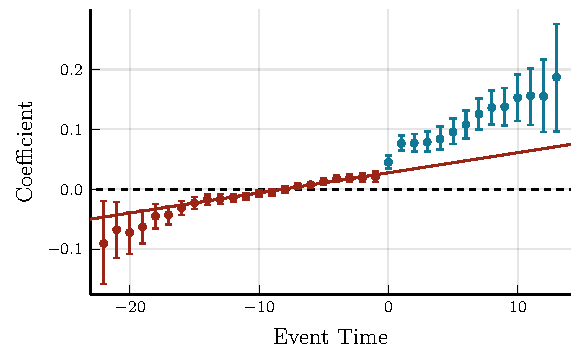
\includegraphics[width = 0.9\textwidth]{../../figures/did2s_retail_bootstrap_1000.pdf}
  \end{figure}
\end{frame}

\begin{frame}{Factor Model}
  Turning to our factor model estimator, we use the following variables at their 1980 baseline values as instruments:
  \begin{itemize}
    \item share of population employed in manufacturing 
    \item shares of population below and above the poverty line
    \item shares of population employed in the private-sector and by the government 
    \item shares of population with high-school and college degrees
  \end{itemize}

  \smallskip\pause
  Think that these are predictive of the kinds of economic trends Walmart may be targeting
  \begin{itemize}
    \item Using baseline values helps us avoid picking up on concurrent shocks that are correlated with walmart opening
  \end{itemize}
\end{frame}

\begin{frame}{Generalized Imputation Estimator}
  \begin{figure}
    \caption{Effect of Walmart on County $\log$ Retail Employment}
    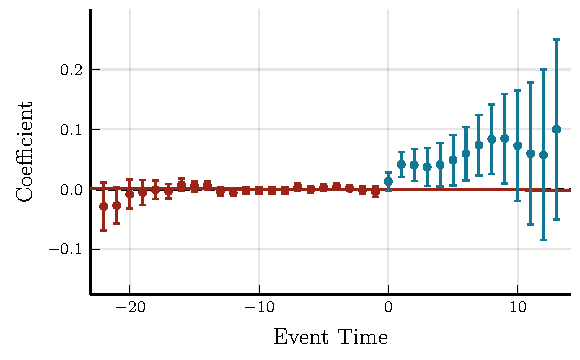
\includegraphics[width = 0.9\textwidth]{../../figures/factor_retail_p_2_bootstrap_1000.pdf}
  \end{figure}
\end{frame}

\begin{frame}{Conclusion}
  \begin{itemize}
    \item Present a fixed-T imputation procedure to identify treatment effects under a factor-model (nesting the TWFE model)
    
    \item Our estimator allows for valid identification of treatment effects when treatment is targeted based on a unit's economic trends.
    
    \item More work to be done on thinking through more explicit connections to VAR and local projection methods \citep{dube2022local,plagborg2021local}
  \end{itemize}
\end{frame}



\end{document}
